\section{Methodology}

% Multiple steps: don't break into subsections - one single pipeline

% Data description set into subsections, but model workflow in one section

% Concern is time - for validation

% Subset of geotiffs counties


% \subsection{Sampling}

% Ideally, land cover classification models should be trained and validated against samples that are representative of the study area. 
% However, under the constraints of limited labeled data, it may be difficult that samples can capture the full range of variation in the study area. 
% Stratified sampling is a common approach to adress this issue, where the study area is divided into strata based on some characeteristic (such as land cover class or sub-region) and samples are drawn from each stratum.
% However, unlike traditional land cover classification models, our semantic segmentation model necessitates the use of densely annotated tiles that exhibit a high degree of diversity with regards to spatial characeteristics.
% Ideally, a single training tile should consist of a mix of land cover classes, and the arrangement of land cover classes should similarly be representative of the study area as a whole.
% In order to achieve this, we employ a stratified sampling strategy that uses the National Land Cover Database (NLCD) to guide the selection of training, validation, and testing tiles such that both the distribution of classes in the tiles is representative of the study area and the content of the tiles is heterogeneous and diverse in terms of spatial characteristics.


% The NLCD provides land cover data at a 30m resolution for the entire United States, and the most recent edition (Annual NLCD) provides yearly land cover data between 19185 and 2023. 
% We use 2023 NLCD data in order to ensure the land cover data is consistent with the NAIP imagery acquired during the same year. 
% For our land cover product, we reclassify the level 1 land cover product to correspond with our choice of legend according to the mapping schema in Table \ref{tab:nlcd-reclass}.
% A grid of 256 m x 256 m square tiles is overlaid over the study area and the proportion of each land cover class is calculated for each cell. 
% Applying principal component analysis (PCA) to the land cover relative frequency data, we identify the first two principal components capture 94.24\% of the data. 
% Figure \ref{fig:ms_pca} visualizes the first two principal components of the land cover data at the tile level --- higher values of the first principal component correspond to a higher proportion of developed land cover classes, while higher values of the second principal component correspond to a higher proportion of forested and herbaceous land cover, with lower values appearing to correlate with regions primarily composed of cultivated crops. 
% Tiles are subsequently into 250 clusters using K-means clustering operating on these two principal components. From each cluster, we sample 2 candidate tiles for training, 1 for validation, and 1 for testing. 
% This results in a total of 500 training tiles, 250 validation tiles, and 250 testing tiles.

% Ensuring this strategy yields high-quality training data that is representative of the study area is crucial to the success of the model. 
% However, we recognize that a rigid evaluation of such an approach to stratification is not possible due to the lack of ground truth data for the study area. 
% One measure we take to ensure the stratification is effective is to inspect the distribution of land cover classes across the splits. 
% Figure \ref{fig:land-cover-distribution} shows that the distribution of land cover classes is consistent across the training, validation, and testing splits, and that these distributions are fairly representative of the study area as a whole. 
% One important note is that the distribution of land cover classes in the study area is highly imbalanced, with the majority of Mississippi's land cover being classified as forest, with a low density of urban and forested areas. 
% In order to tackle this issue, other strategies employ a synthetic oversampling of minority classes or strategic undersampling of majority classes \note{CITE}. 
% Even though our approach to stratifying the data does not explicitly enforce such policies, comparing the land cover class distribution in the sampeled tiles to the distribution across the entire state shows that our sampling strategy achieves a similar outcome to such oversampling and undersampling strategies. 
% Further, our approach tends to avoid sampling tiles that are composed of a single land cover class --- in the original NLCD data, 29.96\% of the tiles are composed of a single land cover class, while only 1.90\% of the sampled tiles are composed of a single land cover class. This is promising, as these homogenous tiles are likely to be less imformative for training the model \note{CITE}. 

\subsection{Sampling}

Ideally, land cover classification models should be trained and validated against samples that are representative of the study area. 
However, under the constraints of limited labeled data, it may be difficult to capture the full range of variation in the study area. 
Stratified sampling is a common approach to address this issue, where the study area is divided into strata based on some characteristic (such as land cover class or sub-region) and samples are drawn from each stratum.
Unlike traditional land cover classification models, our semantic segmentation model necessitates the use of densely annotated tiles that exhibit a high degree of diversity with regards to spatial characteristics.
Ideally, a single training tile should consist of a mix of land cover classes, and the arrangement of land cover classes should similarly be representative of the study area as a whole.
To achieve this, we employ a stratified sampling strategy using the National Land Cover Database (NLCD) to guide the selection of training, validation, and testing tiles.
This ensures that both the distribution of classes in the tiles is representative of the study area and the content of the tiles is heterogeneous and diverse in terms of spatial characteristics.

The NLCD provides land cover data at a 30m resolution for the entire United States, and the most recent edition (Annual NLCD) provides yearly land cover data between 1985 and 2023. 
We use 2023 NLCD data to ensure the land cover data is consistent with the NAIP imagery acquired during the same year. 
For our land cover product, we reclassify the level 1 land cover product to correspond with our choice of legend according to the mapping schema in Table \ref{tab:nlcd-reclass}.

A grid of 256 m x 256 m square tiles is overlaid over the study area, and the proportion of each land cover class is calculated for each cell. 
Applying principal component analysis (PCA) to the land cover relative frequency data, we identify that the first two principal components capture 94.24\% of the data variance. 
Figure \ref{fig:ms_lc_pcs} visualizes the first two principal components of the land cover data at the tile level.
Higher values of the first principal component correspond to a higher proportion of impervious land cover types in each tile, while higher values of the second principal component correspond to a higher proportion of forested and herbaceous land cover, with lower values correlating with regions that consist of tiles primarily or wholly composed of cultivated crops.
These tiles are subsequently grouped into 250 clusters using K-means clustering operating on these two principal components. 
As shown in Figure \ref{fig:clusters}, the clustering algorithm effectively divides the principal component space into regions that correspond to differing land cover compositions.
From each cluster, we sample 2 candidate tiles for training, 1 for validation, and 1 for testing.
This results in a total of 500 training tiles, 250 validation tiles, and 250 testing tiles.

\begin{figure}[ht]
    \centering
    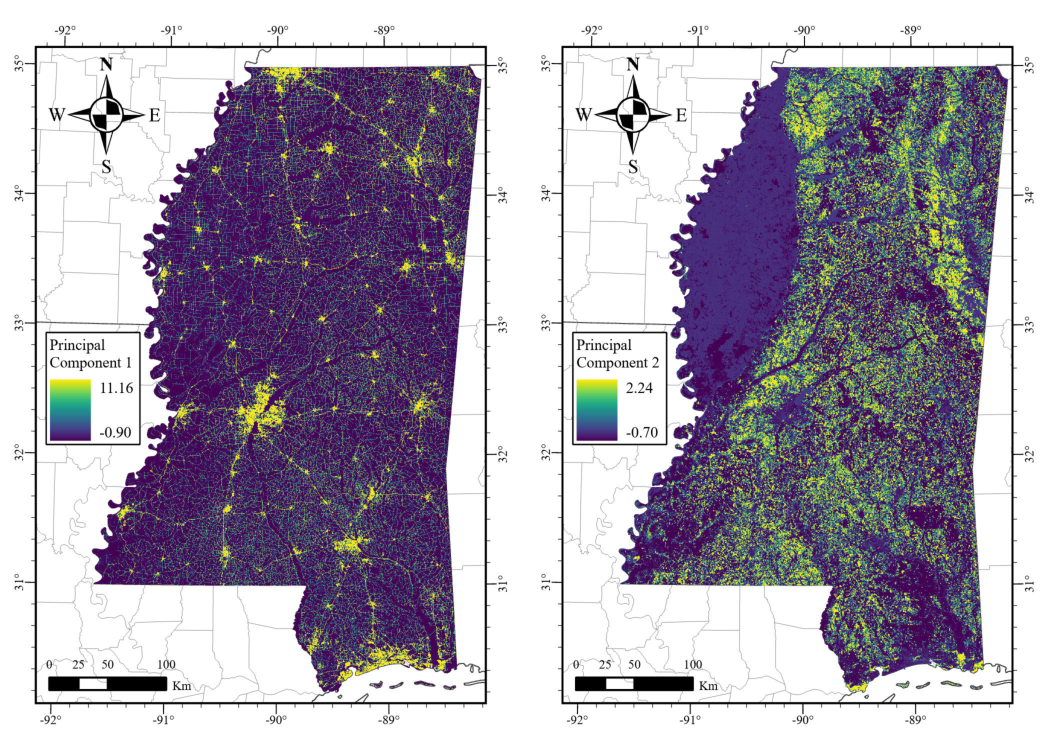
\includegraphics[width=\textwidth]{images/sampling/Mississippi_PCs.pdf}
    \caption{Principal components of NLCD relative frequencies per candidate tile.}\label{fig:ms_lc_pcs}
\end{figure}

\begin{figure}[ht]
    \centering
    
\includegraphics[width=0.8\textwidth]{images/sampling/clusters_250.png}
    \caption{Clusters from which samples are draw in principal component space.}\label{fig:clusters}
\end{figure}

\begin{figure}[H]
    \centering
    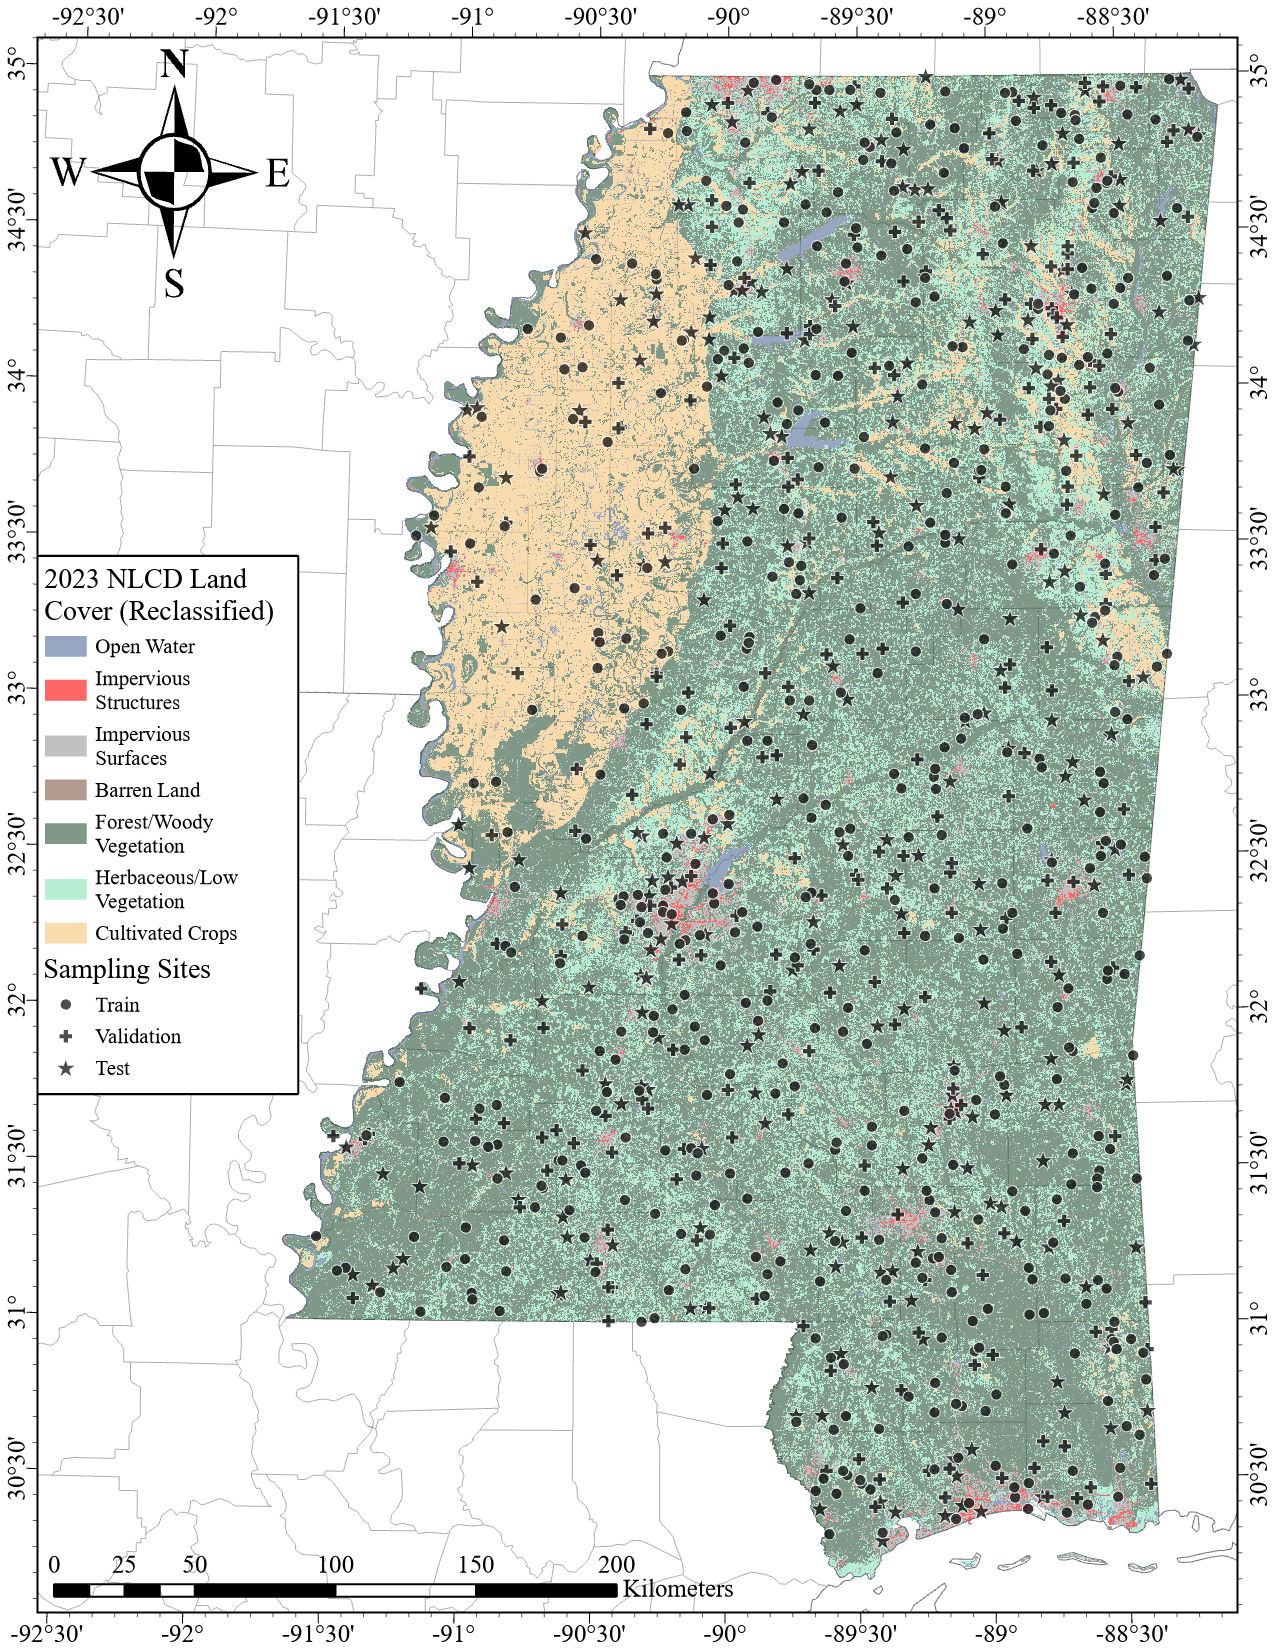
\includegraphics[height=0.9\textheight]{images/sampling/sampling_sites_map.pdf}
    % \vspace{-0.75cm}
    \caption{Sample locations for the Mississippi dataset.}\label{fig:sample_locations}
\end{figure}

Ensuring this strategy yields high-quality training data that is representative of the study area is crucial to the success of the model.
However, we recognize that a rigid evaluation of such an approach to stratification is not possible due to the lack of ground truth data for the study area.
One measure we take to ensure the stratification is effective is to inspect the distribution of land cover classes across the splits. Figure \ref{fig:land-cover-distribution} shows that the distribution of land cover classes is consistent across the training, validation, and testing splits, which is ideal for ensuring that the model is exposed to a representative sample of the study area's land cover diversity.
One important note is that the distribution of land cover classes in the study area is highly imbalanced, with the majority of Mississippi's land cover being classified as forest, and a low density of urban and developed areas. 
To tackle this issue, other strategies often employ synthetic oversampling of minority classes or strategic undersampling of majority classes \note{CITE}. 
Although our approach to stratifying the data does not explicitly enforce such policies, comparing the land cover class distribution in the sampled tiles to the distribution across the entire state (as shown in Figure \ref{fig:land-cover-distribution}) demonstrates that our sampling strategy achieves a similar outcome to these oversampling and undersampling strategies.
Furthermore, our approach tends to avoid sampling tiles that are composed of a single land cover class. 
In the original NLCD data, 29.96\% of the tiles are composed of a single land cover class, while only 1.90\% of the sampled tiles are composed of a single land cover class. This is promising, as these homogeneous tiles are likely to be less informative for training the model \note{CITE}.
% Further, our approach tends to avoid sampling tiles that are composed of a single land cover class. 
% In the original NLCD data, 29.96\% of the tiles are composed of a single land cover class, while only 1.90\% of the sampled tiles are composed of a single land cover class. This is promising, as these homogeneous tiles are likely to be less informative for training the model \note{CITE}.



\subsection{Model configuration}

Our model is baed on the U-Net architecture, which is a popular choice for semantic segmentation tasks due to its relatively simple yet effective design \cite{ronnebergerUNetConvolutionalNetworks2015e} \note{OTHERS!!!}.
First, in lieu of the original convolutional encoder network in the original implementation, we employ a much deeper ResNet-152 network as the encoder.
Our reasoning for this choice is that the increased number of layers in the ResNet-152 network will facilitate more complex feature extraction, particularly during the self-supervised pre-training phase, where the large amount of unlabeled data will allow the encoder to learn to capture rich representations of spatial features in the input imagery.
The number of channels accepted and produced by the decoder convolutions are subsequently adjusted to match the output of their corresponding encoder blocks.
Second, we replace the transposed convolutional layers in the original U-Net decoder with bilinear upsampling to reduce the presence of checkerboard artifacts in the upsampled feature maps, which can inhibit the quality of the output segmentation maps \cite{odenaDeconvolutionCheckerboardArtifacts2016, sanjarImprovedUNetFully2020}.
Finally, in each decoder block, we introduce a residual connection between the output of the first convolutional layer and the output of the second convolutional layer to facilitate the flow of information through the network and improve training stability \cite{heDeepResidualLearning2016c}.

% 1) the encoder network is a ResNet-152 convolutional network, 2) the decoder blocks do not use transposed convolutions, and instead use bilinear upsampling followed by 2 3x3 convolutions, 3) within each decoder block, a residual connection is added between the output of the first convolution and the output of the second convolution, and 4) after the final decoder block, an additional 2 3x3 convolutions (also with residual connections) operate on the full resolution feature maps prior to the final 1x1 convolutional layer. \note{COMPLETE ME!} 

\subsection{Pre-training}

Our pre-training approach consists of two phases: a self-supervised pre-training phase and a fully supervised pre-training phase.

\paragraph{Self-supervised pre-training}
% In the first stage, we construct a simple denoising convolutional autoencoder by resampling feature maps from each stage of the ResNet-152 encoder to the original input resolution, concatenating them, and passing them through a single 1\(\times\)1 convolutional layer to produce an output with the same dimensions as the input.
In the first stage of pre-training, we train a denoting autoencoder using the unannotated NAIP imagery over the state of Mississippi.
Our denoising autoencoder consists of a ResNet-152 encoder network and a simple decoder network that receives feature maps from each stage of the encoder network, resamples them to the original input resolution using bilinear interpolation, concatenates them, and passes them through a single 1\(\times\)1 convolutional layer to produce an output with the same dimensions as the input.
The ResNet-152 encoder network is initialized with ImageNet-1k pre-trained weights, while the decoder network is randomly initialized.
A full decoder network (as is common in traditional autoencoders) is not used in this phase, as our primary goal is to force the encoder network to learn robust features present in the imagery that are necessary for reconstruction, rather than to necessarily learn to denoise the input images with a high degree of accuracy.
Further, a U-Net architecture (like the one used in the subsequent fully supervised stages of training) are not used, as the presence of skip connections in the network can inhibit strong representation learning in the encoder network
The single-layer decoder network is designed to ensure that backpropagation primarily influences the parameters of the encoder network
% To reduce the computational cost of pre-training the model during this phase, images are randomly cropped to 96\(\times\)96 pixels before being passed through the model.

Two types of noise are added to the image: Gaussian noise and Poisson noise.
The intensity of the Gaussian noise is controlled by the standard deviation parameter \(\sigma\), which is randomly sampled from a uniform distribution \(U(0, 2)\).
Similarly, the intensity of the Poisson noise is controlled by the rate parameter \(\lambda\), which is also randomly sampled from a uniform distribution \(U(0, 1)\). 
Since random variables sampled from a Poisson distribution are strictly non-negative, Poisson noise is both added and subtracted from the input image (using the same \(\lambda\) value) to increase the impact of the noise on the input image.
% Our implementation is distinct from other denoising autoencoders in that the amount and type of noises added to an image is random, and not a fixed amount \note{CITE!!!}.
% Ideally, while this may inhibit the model's ability to effectively denoise an image, it will force the model to learn robust features that are invariant to the type and amount of noise present in the input image \note{CITE!!!???}.
Model inputs are standardized to have zero mean and unit variance on a per-band basis using the mean and standard deviation of the pre-training data prior to adding noise.
We opt for a relatively small batch size of 8 to reduce the memory requirements of the model during pre-training and to better approximate the stochasticity of the training data, improving the model's generalization ability --- an important consideration given our goal of transfering the encoder network to a downstream task \cite{keskarLargeBatchTrainingDeep2017, mastersRevisitingSmallBatch2018}.
The loss function used during this self-supervised pre-training phase the mean absolute error between the model's raw output and the normalized input image.
While the mean squared error is a common choice for autoencoder models, we opt for the mean absolute error as it tends to produce sharper images in the output \cite{zhaoLossFunctionsImage2017,mustafaTrainingTaskSpecificImage2022}.
The AdamW optimizer is used to train the model, with an initial learning rate of 1e-6 and a weight decay of 1e-2 \cite{loshchilovDecoupledWeightDecay2019}.
After each epoch of pre-training, the model is evaluated using the pre-training validation set to ensure that the model is fitting the data properly and to adjust the learning rate if necessary.
If the validation loss does not decrease after an epoch, the learning rate is reduced by a factor of 0.1.
While such a scheduler is aggressive, given the large volume of samples in the pretraining dataset and the sheer number of parameter updates that occur within a single epoch, we find that the model tends to optimize quickly and that there is little benefit to continuing to train at a learning rate where previous epochs have not shown improvement.
Further, if the pretraining validation loss does not decrease for 5 consecutive epochs, the pre-training phase is terminated early.
As such, while the model is trained for a maximum of 100 epochs, our model is capable of converging in 9 epochs \note{ADD FIGURE FOR PRE-TRAINING LOSS CURVE}.
In order to estimate the quality of the reconstructions, we track the peak signal-to-noise ratio (PSNR) and structural similarity index (SSIM) between the input and output images during training \cite{horeImageQualityMetrics2010}.

\note{FIGURE: DIFFERENT TYPES OF NOISE}


\paragraph{Fully supervised pre-training}

Once the self-supervised pre-training phase is complete, the encoder network is used as the encoder in the U-Net architecture, and the decoder network is initialized with random weights.
% Oversampling strategy
% In order to increase the diversity of the training data, oversampling is employed in this stage. If a tile contains a minority class in greater proportion that the average proportion 
% \note{TODO: Describe oversampling strategy} - under this strategy, minority classes are defined as any class comprising less than \note{X.XX}\% of the total pixels in the training set.
% If a tile contains a minority class that is in greater proportion that the relatvie frequency of that class in the training set, then the tile is duplicated \note{X} times.
The model is trained to minimize the Focal loss, defined as:
\begin{equation}
    \mathcal{L}_{\text{Focal}}\left( p_c \right) = 
    \begin{cases}
        -\alpha_c \left(1 - p_c\right)^\gamma \log\left(p_c\right) & \text{if } y = c \\
        -\left(1 - \alpha_c\right) p_c^\gamma \log\left(1 - p_c\right) & \text{otherwise}
    \end{cases}
\end{equation}
where \(p_c\) is the predicted probability of class \(c\), \(y\) is the true class label, \(\alpha_c\) is the class weight for class \(c\), and \(\gamma\) is a hyperparameter that controls the degree of class weighting.
In order to address the class imbalance present in the data (\note{REFERENCE FIGURE HERE}, we employ a class weighting strategy that assigns class weights according to the formula:
\begin{equation}
    \alpha_c = \frac{\left(1 - \rho_c\right)^\beta}{\sum_{c=1}^{C} \left(1 - \rho_c\right)^\beta}
    \label{eq:class_weight}
\end{equation}
where \(\rho_c\) is the proportion of class \(c\) in the training set, \(\beta\) is a hyperparameter that controls the degree of class weighting, and \(C\) is the total number of classes.
For our experiments, we set \(\gamma = 2.0\) in accordance with the authors' findings in the original Focal loss paper \cite{linFocalLossDense2017}, and \(\beta=2.0\) such that minority classes are emphasized without majority classes being under-represented in the loss function.
Like the previous pre-training stage, the model's parameters are updated using the AdamW optimizer, with an initial learning rate of 
Like the previous pre-training stage, the model is evaluated after every epoch using the validation set to adjust the learning rate and terminate the training early if necessary: if no improvement is observed in the validation loss for 3 consecutive epochs, the learning rate is reduced by a factor of 0.1, and if no improvement is observed for 15 consecutive epochs, the training is terminated early.

The model 


\subsection{Fine-tuning}

\subsection{Inference}

Once the models have been trained and evaluated, they are 

\subsection{Evaluation}